%=== CHAPTER THREE (3) ===
%=== (Actual work done and contribution, including literature survey) ===

\chapter{Research Methodology}
\label{ch:methodology}
\begin{spacing}{2.0}


\section{Introduction to the Methodology}
This chapter delineates the software architecture and technical realisation of the purely spatiotemporal deep learning framework developed for automated detection of traffic anomalies. Constructed entirely in Python, the system utilises the OpenCV library for deterministic kinematic extraction and the PyTorch framework for probabilistic deep learning pattern recognition.

In contrast to conventional methodologies that depend on sequential spatial tracking and bounding boxes, this framework entirely foregoes discrete object detection. Instead, anomaly classification is performed through the direct interpretation of the scene’s unstructured kinetic energy. This is achieved by producing dense optical flow heatmaps and subsequently mapping them via a custom-trained ResNet-18 classifier, thereby enabling the neural network to explicitly learn the physical signatures of an impact.

To attain high-performance throughput suitable for real-world deployment, a multi-threaded, headless video processing architecture was developed. To circumvent the Global Interpreter Lock (GIL) and sustain optimal processing speeds during intensive inference workloads, an asynchronous producer-consumer model was employed. Additionally, by assessing raw kinetic energy instead of high-resolution spatial identifiers, the framework inherently complies with data privacy regulations (GDPR), providing a highly secure surveillance solution without reliance on computationally demanding visual obfuscation techniques.

\begin{figure}[H]
    \centering
    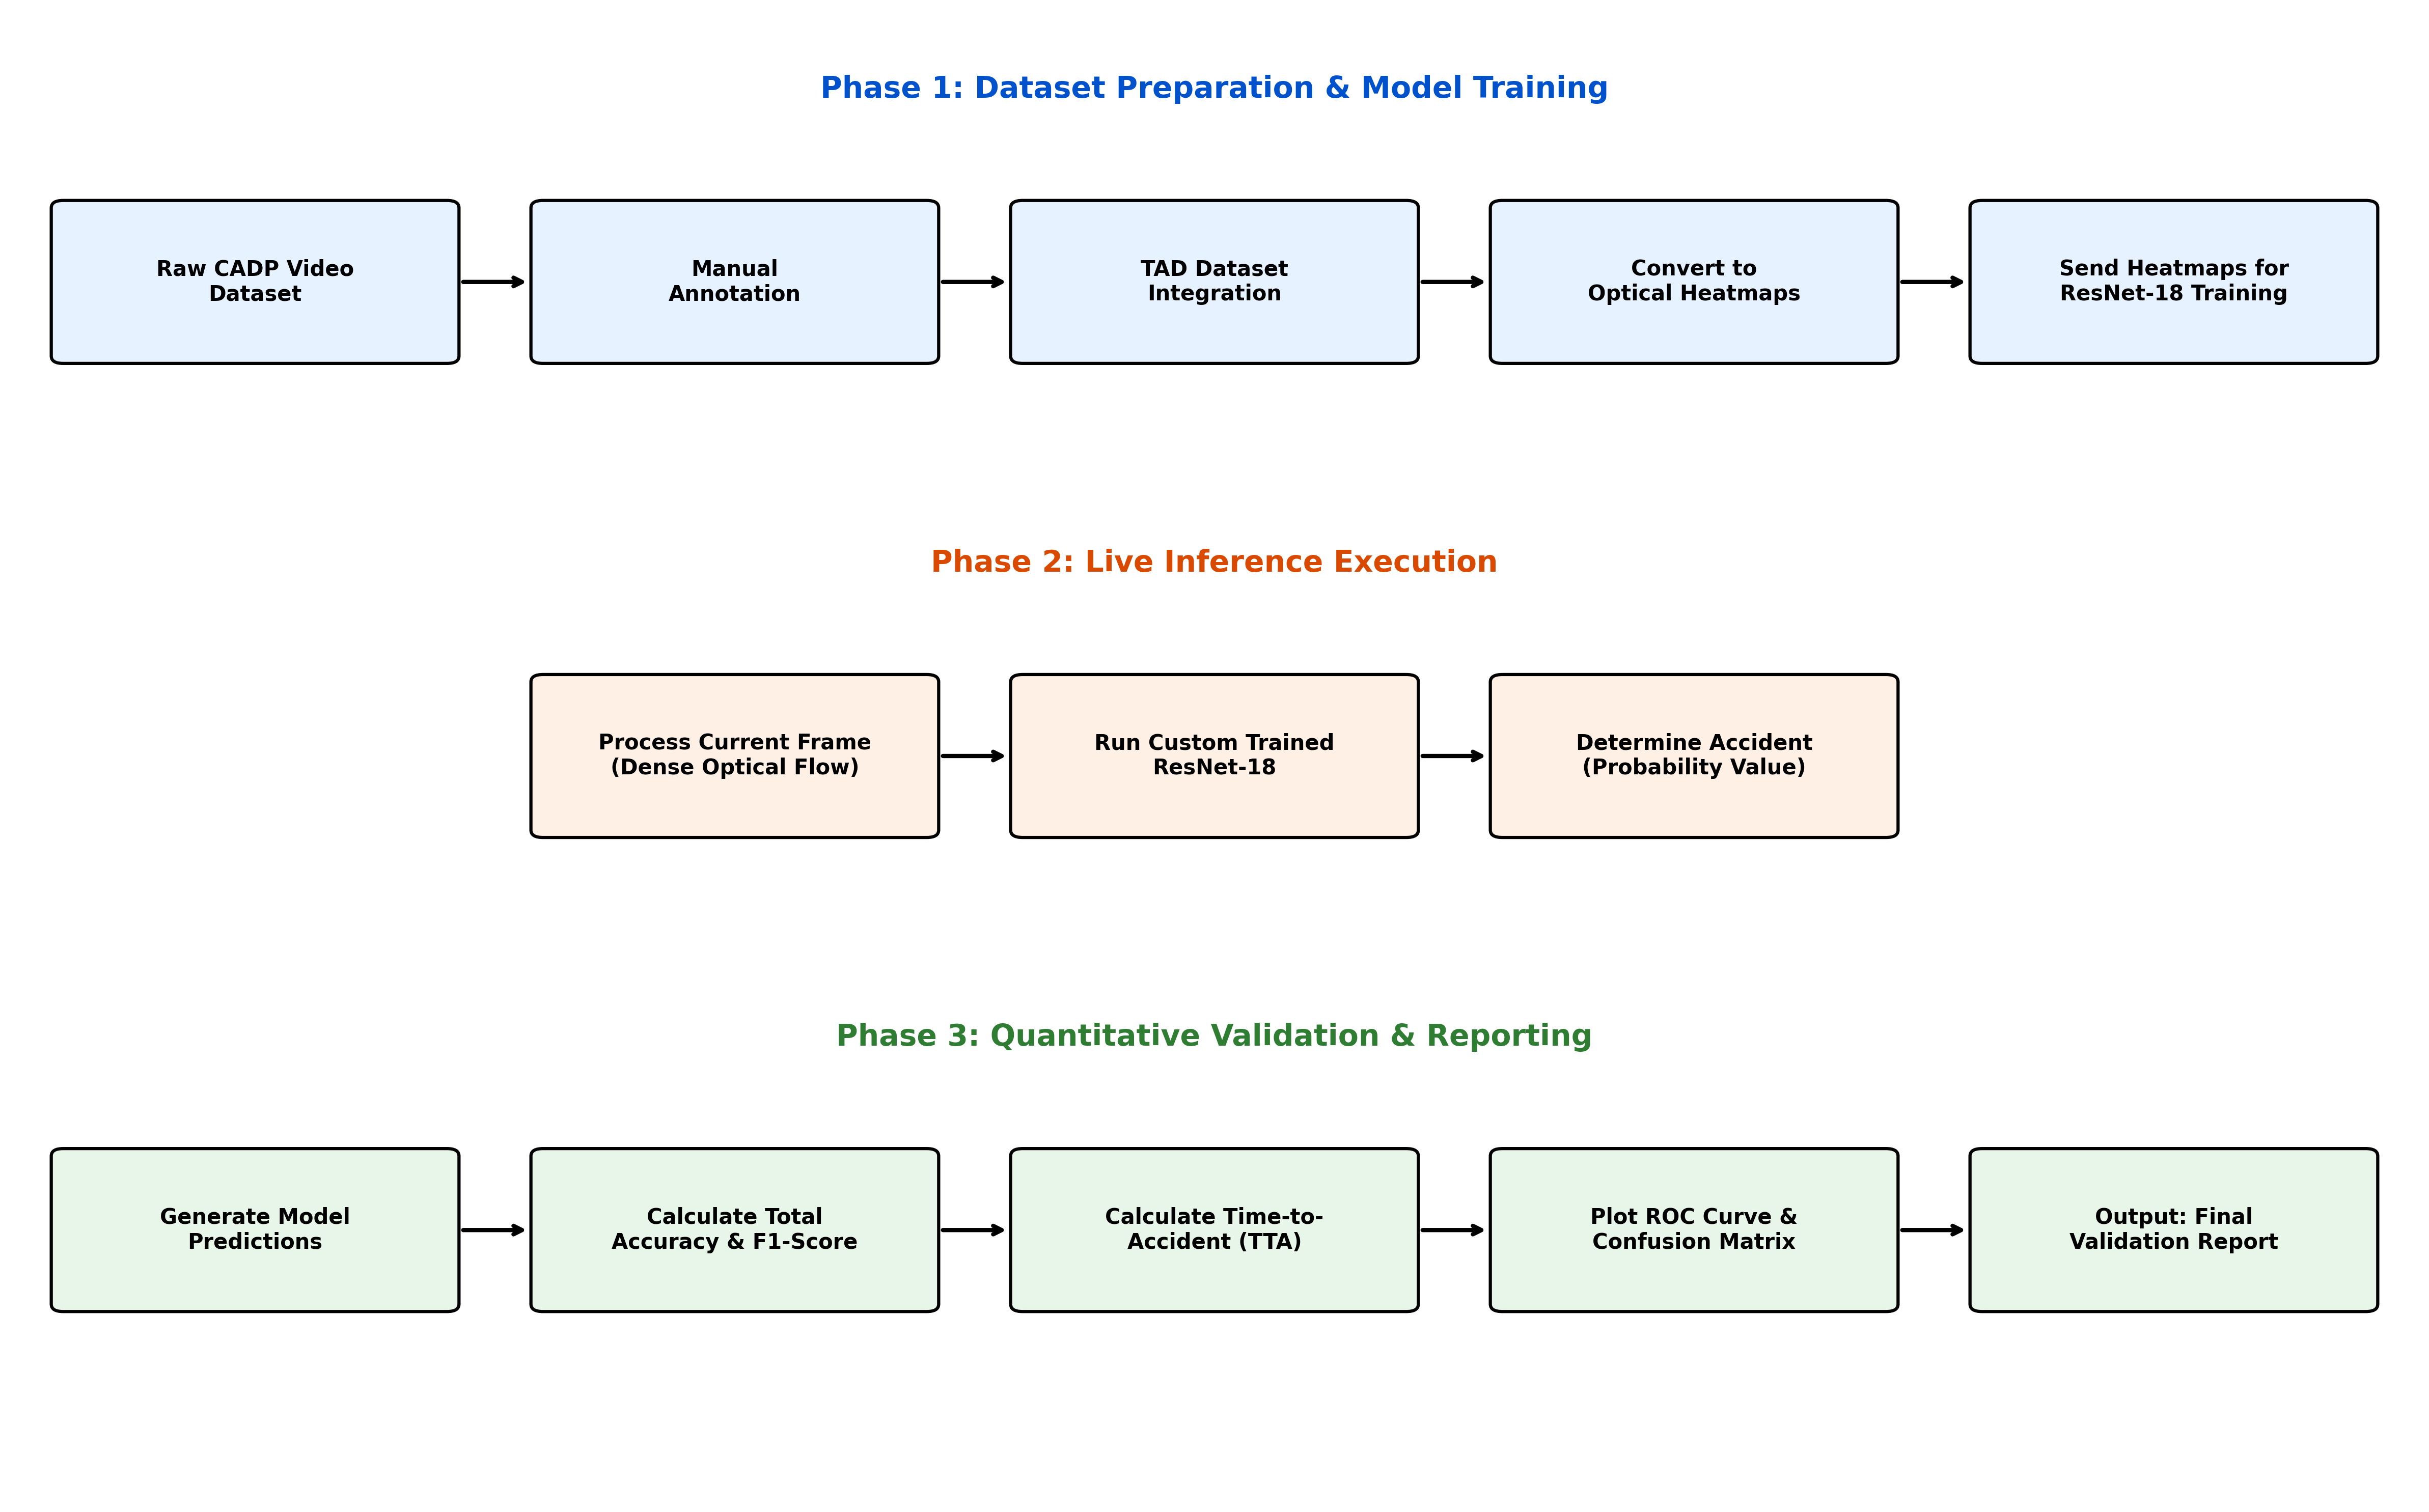
\includegraphics[width=0.8\textwidth]{Figures/simple_pipeline.png}
    \caption{A high-level pipeline diagram illustrating the purely spatiotemporal architecture.}
    \label{fig:simple_pipeline}
\end{figure}

\section{Data Engineering, Harmonisation, and Mathematical Balancing}
The deep learning component of the purely spatiotemporal pipeline necessitated a robust, custom-built data engineering workflow to ensure the PyTorch classifier received highly structured training data. To train the spatial-temporal features of the system, the Car Accident Detection and Prediction (CADP) benchmark dataset was utilised as the primary data source, from which raw CCTV video clips of real-world collisions were extracted.

Given that the CADP dataset consists almost entirely of positive accident events, the raw data distribution was heavily skewed. To process this, a custom annotation tool was developed to facilitate the manual review of video files. Precise temporal markers denoting the exact frames of collisions were identified and logged into structured records. Following this annotation phase, an automated data cleaning pipeline was implemented to rigorously pre-process the dataset. This pipeline parsed the recorded temporal data and systematically evaluated visual fidelity, automatically purging any low-resolution, unsuitable, or heavily obscured footage to prevent the introduction of noise into the neural network.

While this programmatic refinement substantially enhanced the precision of the ground truth labels, executing the automated splitting logic (\texttt{split\_data.py}) to partition the data for training and validation revealed a critical structural vulnerability: a severe deficiency of "normal" baseline traffic frames.

To mitigate this bias and introduce the necessary baseline frames, 250 high-definition, incident-free videos from the Traffic Anomaly Detection (TAD) dataset were incorporated. The TAD videos were converted into dense optical flow heatmaps using the exact same OpenCV Farnebäck parameters applied to the CADP dataset, and the outputs of both datasets were merged. This architectural decision significantly reduced false positives and guaranteed that the final classifier activates exclusively in the presence of genuine kinetic anomalies.

\begin{table}[H]
    \centering
    \begin{tabular}{p{3cm} p{3cm} p{4cm} p{4cm}}
        \toprule
        \textbf{Dataset Constituent} & \textbf{Source Benchmark} & \textbf{Primary Content} & \textbf{Post-Processing Application} \\
        \midrule
        Anomalous Frames & CADP Dataset & Vehicle Collisions, Skidding & Temporal annotation to extract precise impact frames. \\
        Normal Frames & TAD Dataset & Standard Traffic Flow & Generation of optical flow baselines to balance the class distribution. \\
        Validation Set & CADP \& TAD & Mixed Scenarios & Evaluated to quantify classification performance and verify the reduction of the False Positive Rate (FPR). \\
        \bottomrule
    \end{tabular}
    \caption{Summary of Database Constituents and Sources}
    \label{tab:database_sources}
\end{table}

\section{Handling Dataset Imbalance via Dataset Merging}
A principal challenge in the training of spatiotemporal neural networks for anomaly detection resides in the inherent class imbalance characteristic of real-world surveillance data. Traffic collisions are exceedingly infrequent events in comparison to the extensive continuum of routine driving activities. When a model is trained on such a skewed distribution, it tends to converge upon a suboptimal local minimum, disproportionately favouring the prediction of the majority class (normal traffic) to artificially maximise its overall accuracy, thereby failing entirely to identify genuine accidents.

To overcome this limitation and develop a mathematically balanced training environment, a meticulous data engineering pipeline was implemented. The primary source of anomalous kinetic data was the Car Accident Detection and Prediction (CADP) dataset. However, given that each CADP video contains several seconds of routine driving prior to the collision, the dataset could not be utilised in its entirety. Instead, a manual temporal annotation process was conducted. Each video clip within the CADP dataset was individually reviewed, and the precise frames capturing the moment of structural impact and immediate kinetic deformation were explicitly isolated. These specific ‘accident frames’ were systematically separated from the preceding ‘normal frames’, ensuring that the neural network would only learn the pure physical signature of a collision.

Despite this rigorous extraction, the number of isolated accident frames markedly exceeded the available normal frames within the CADP repository. To achieve balance and prevent the network from producing elevated false-positive rates, the dataset was augmented by incorporating routine driving footage from the independent Traffic Anomaly Detection (TAD) dataset. A programme was employed to iteratively generate dense optical flow heatmaps from the TAD videos until precisely 19,200 'normal' spatiotemporal tensors were extracted. By combining the explicitly annotated impact points from CADP with the extensive repertoire of steady-state flow data from TAD, the final training dataset was rendered perfectly balanced. This equal class distribution compelled the ResNet-18 architecture to genuinely learn the intricate spatiotemporal boundaries that distinguish routine traffic flow from catastrophic kinetic anomalies.

\section{Mathematical Formulation of Dense Optical Flow}
As indicated in the literature, the assessment of the kinetic energy involved in a traffic incident necessitates the continuous mapping of pixel displacement within a spatial domain. To this end, the methodology proposed herein utilised Gunnar Farnebäck’s dense optical flow algorithm, which employs quadratic polynomial expansion to approximate the local image signal in the vicinity of each pixel. By comparing the polynomial coefficients of consecutive frames, the algorithm computes a dense vector field that delineates both the direction and magnitude of movement for every pixel.

To operationalise this mathematical framework, an automated extraction pipeline was devised utilizing the OpenCV computer vision library. Initially, successive raw RGB video frames were ingested and meticulously standardised to a spatial resolution of $640 \times 360$ pixels. This reduction in dimensions was essential to standardise the coordinate space across various camera feeds and to optimise the computational efficiency for the subsequent neural network. Subsequently, the frames were converted to greyscale, as the Farnebäck algorithm assesses shifts in pixel intensity rather than colour variation.

The dense optical flow was subsequently computed using carefully selected hyperparameters to ensure sensitivity to the rapid physical dynamics characteristic of vehicular collisions. A pyramid scale of 0.5 across three pyramid levels enabled the algorithm to track swiftly moving objects at different resolutions, whilst a window size of 15 pixels offered adequate contextual smoothing to capture the substantial structural deformations typical of a crash.

Once the raw Cartesian displacement vectors (X and Y pixel shifts) were computed, they were mathematically converted into polar coordinates to ascertain the precise angle and magnitude of the local kinetic energy. A key methodological aspect of this process involved the implementation of a rigid noise-filtering threshold. Any pixel displacement with a magnitude of less than 3.0 was forcibly set to zero. This measure effectively distinguished authentic vehicular movement from extraneous environmental noise, such as minor camera vibrations induced by wind impacting the CCTV mounting poles.

Finally, this filtered polar data was transformed into a dense visual heatmap utilising the Hue, Saturation, and Value (HSV) colour space. The angle of movement was mapped to the Hue channel to denote direction, whilst the magnitude was significantly scaled (by a factor of 10.0) and assigned to the Value channel to represent kinetic intensity. Importantly, the Saturation channel was entirely omitted from modification and fixed at a constant maximum value of 255. This structural choice effectively converted the unstructured kinetic physics of a collision into a highly compacted spatiotemporal tensor, explicitly tailored for deep learning classification.

\section{Spatiotemporal Kinetic Energy Mapping via Dense Optical Flow}
Whilst traditional bounding boxes attempt to track individual vehicle trajectories, they inherently fail to capture the unstructured spatial chaos and violent kinetic motion that defines a collision. To quantify this unstructured motion, dense optical flow was implemented using OpenCV's Farnebäck algorithm. Rather than detailing the underlying polynomial mathematics, this section focuses strictly on the algorithm's programmatic integration within the primary processing thread.

During execution, the raw camera feed is continuously converted into a greyscale matrix and compared against the preceding frame. The Farnebäck algorithm computes raw motion vectors in Cartesian coordinates for every pixel. To process this computationally, these vectors are converted into polar coordinates to extract the Euclidean magnitude and angular direction of the physical movement.

To prevent background environmental noise, such as pedestrians or moving foliage, from overwhelming the downstream AI classifier, a static Region of Interest (ROI) mask was implemented. Array slicing was utilised to explicitly enforce a zero-magnitude value on all motion vectors originating outside the carriageway boundaries. Furthermore, a strict noise floor was established, programmatically zeroing out any pixel magnitudes below 3.0 to eliminate minor camera jitter.

Once filtered, these physical motion metrics are encoded into a pre-allocated HSV (Hue, Saturation, Value) matrix buffer. The physical angle of the motion dictates the Hue, whilst the dynamically clipped and scaled magnitude dictates the Value. Finally, this buffer is converted into a standard BGR image array, generating a spatiotemporal heatmap of the scene's kinetic energy. This resulting visual tensor is immediately pushed into a thread-safe queue for asynchronous processing by the deep learning classifier.

\begin{figure}[H]
    \centering
    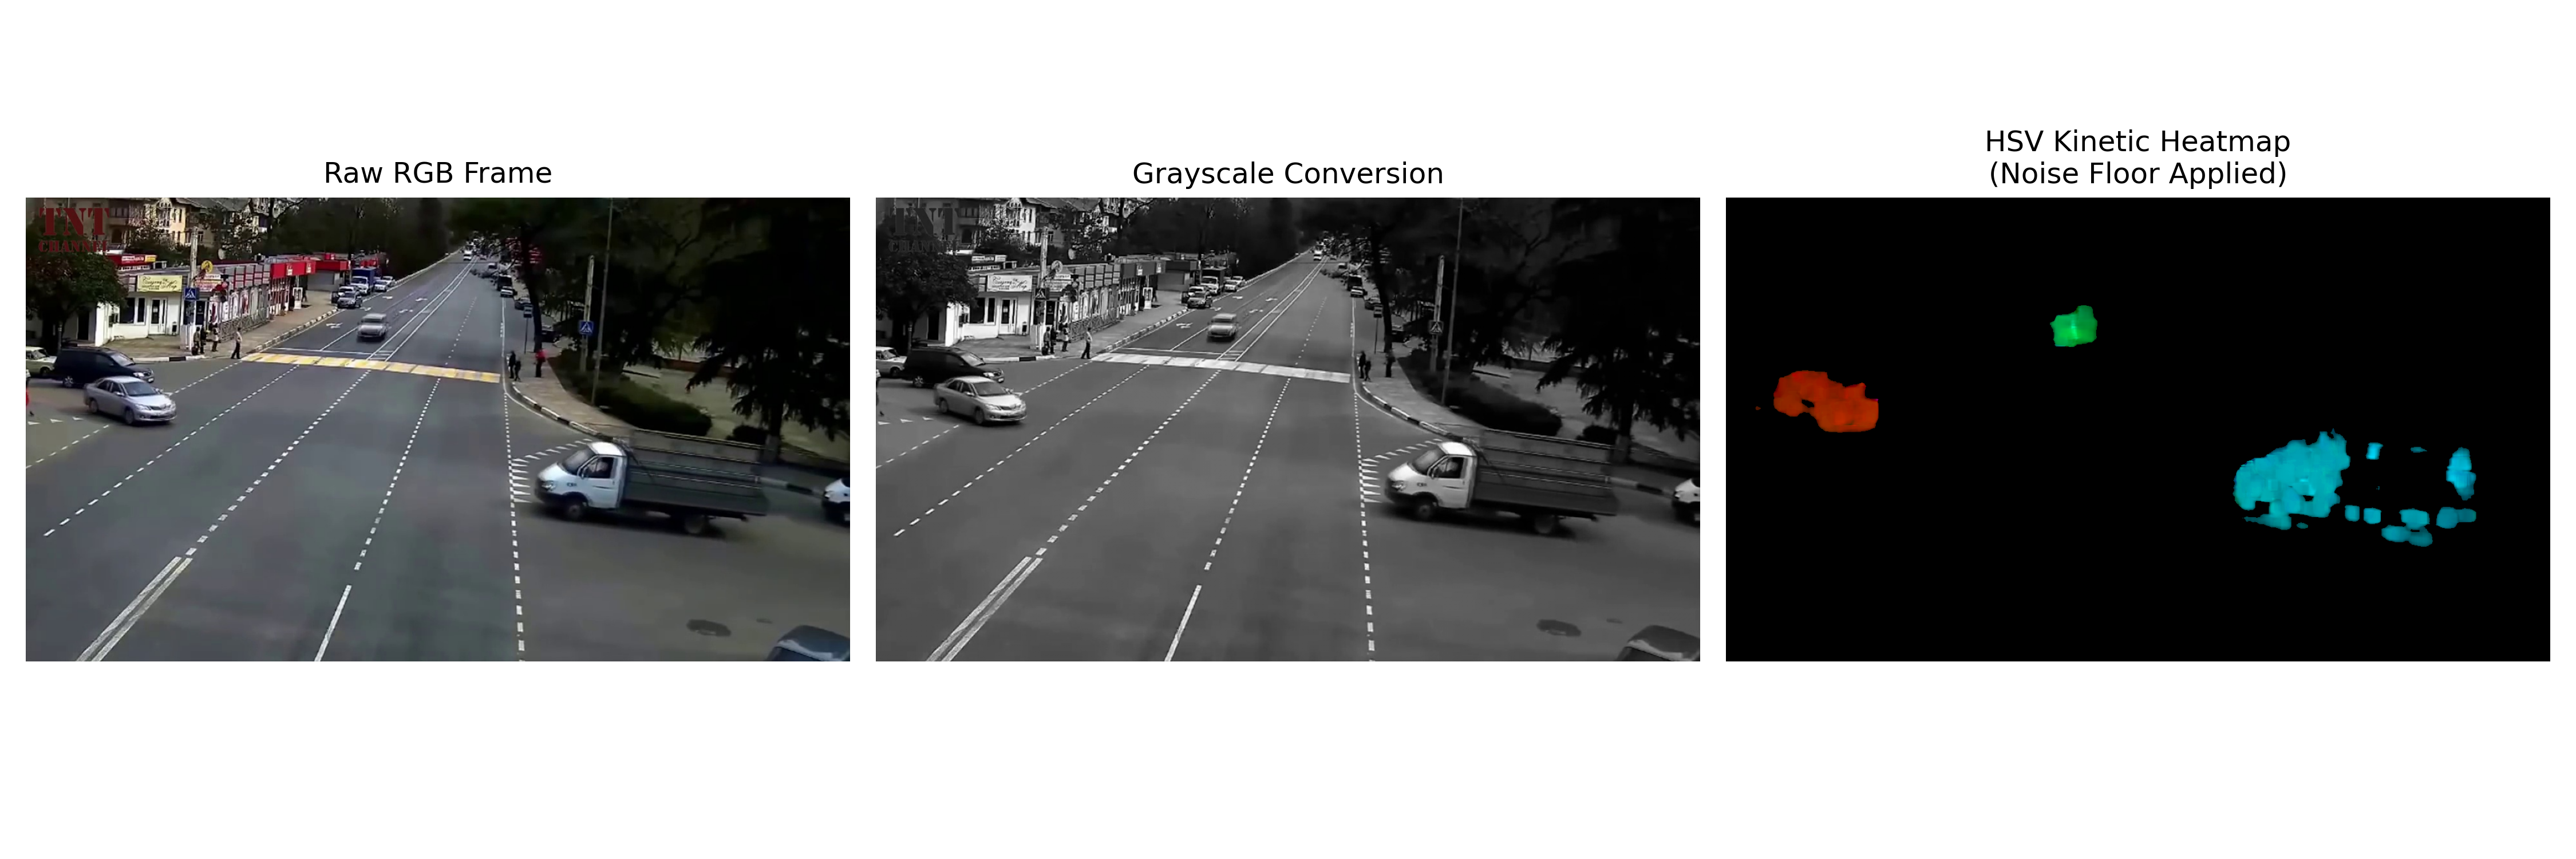
\includegraphics[width=0.9\textwidth]{Figures/tensor_creation.png}
    \caption{A progressive visual of the tensor creation process. Left: Raw RGB frame. Centre: Grayscale conversion. Right: The resulting HSV Heatmap representing kinetic energy, demonstrating the effectiveness of the strict noise floor threshold in blacking out static background.}
    \label{fig:tensor_creation}
\end{figure}

\section{Customisation of the ResNet-18 Architecture}
To classify the extracted kinetic heatmaps, a deep learning architecture grounded in the ResNet-18 framework was employed. Instead of training a neural network from scratch this approach utilised transfer learning. The network was initialised with pre-trained weights derived from prior training on the ImageNet dataset. To maintain this inherent spatial feature extraction capability, the base convolutional layers were 'frozen' during the initial stages of training, thereby preventing the foundational gradient information from being significantly overwritten during optimisation.

A critical methodological adjustment was necessitated to align the network’s input expectations with the nature of the optical flow data. The standard ResNet-18 architecture is fundamentally designed to process three-channel RGB (Red, Green, Blue) spatial images. However, the optical flow heatmaps generated by the system operate within the Hue, Saturation, and Value (HSV) colour space, wherein the Saturation channel was artificially fixed at a constant maximum value of 255. As a result, although the network ingested a three-channel tensor, the underlying data variability was effectively bipartite: the Hue channel represented the angle of the kinetic trajectory, whilst the Value channel encoded the magnitude of kinetic energy.

By effectively providing the network with a two-channel kinetic pseudo-tensor devoid of static visual textures, the convolutional layers were compelled to learn purely spatiotemporal relationships, thereby rendering the system invariant to variations in vehicle colour or environmental illumination. Furthermore, the standard ResNet-18 architecture concludes with a fully connected (FC) layer comprising 1000 nodes, intended for broad object categorisation. This layer was entirely removed and replaced with a customised, lightweight classification head specifically designed for binary anomaly detection.

The customised head incorporates a linear layer that reduces the high-dimensional feature maps to 256 nodes, followed by a Rectified Linear Unit (ReLU) activation function to model non-linear kinetic patterns. A Dropout layer was added with a probability of 0.5, randomly disabling half of the nodes during training to prevent the network from memorising the training data (overfitting). Finally, the architecture culminates in a single-node output layer, paired with a Sigmoid activation function to compress the final tensor into a binary probability metric ranging from 0.0 (Normal) to 1.0 (Accident).

\begin{figure}[H]
    \centering
    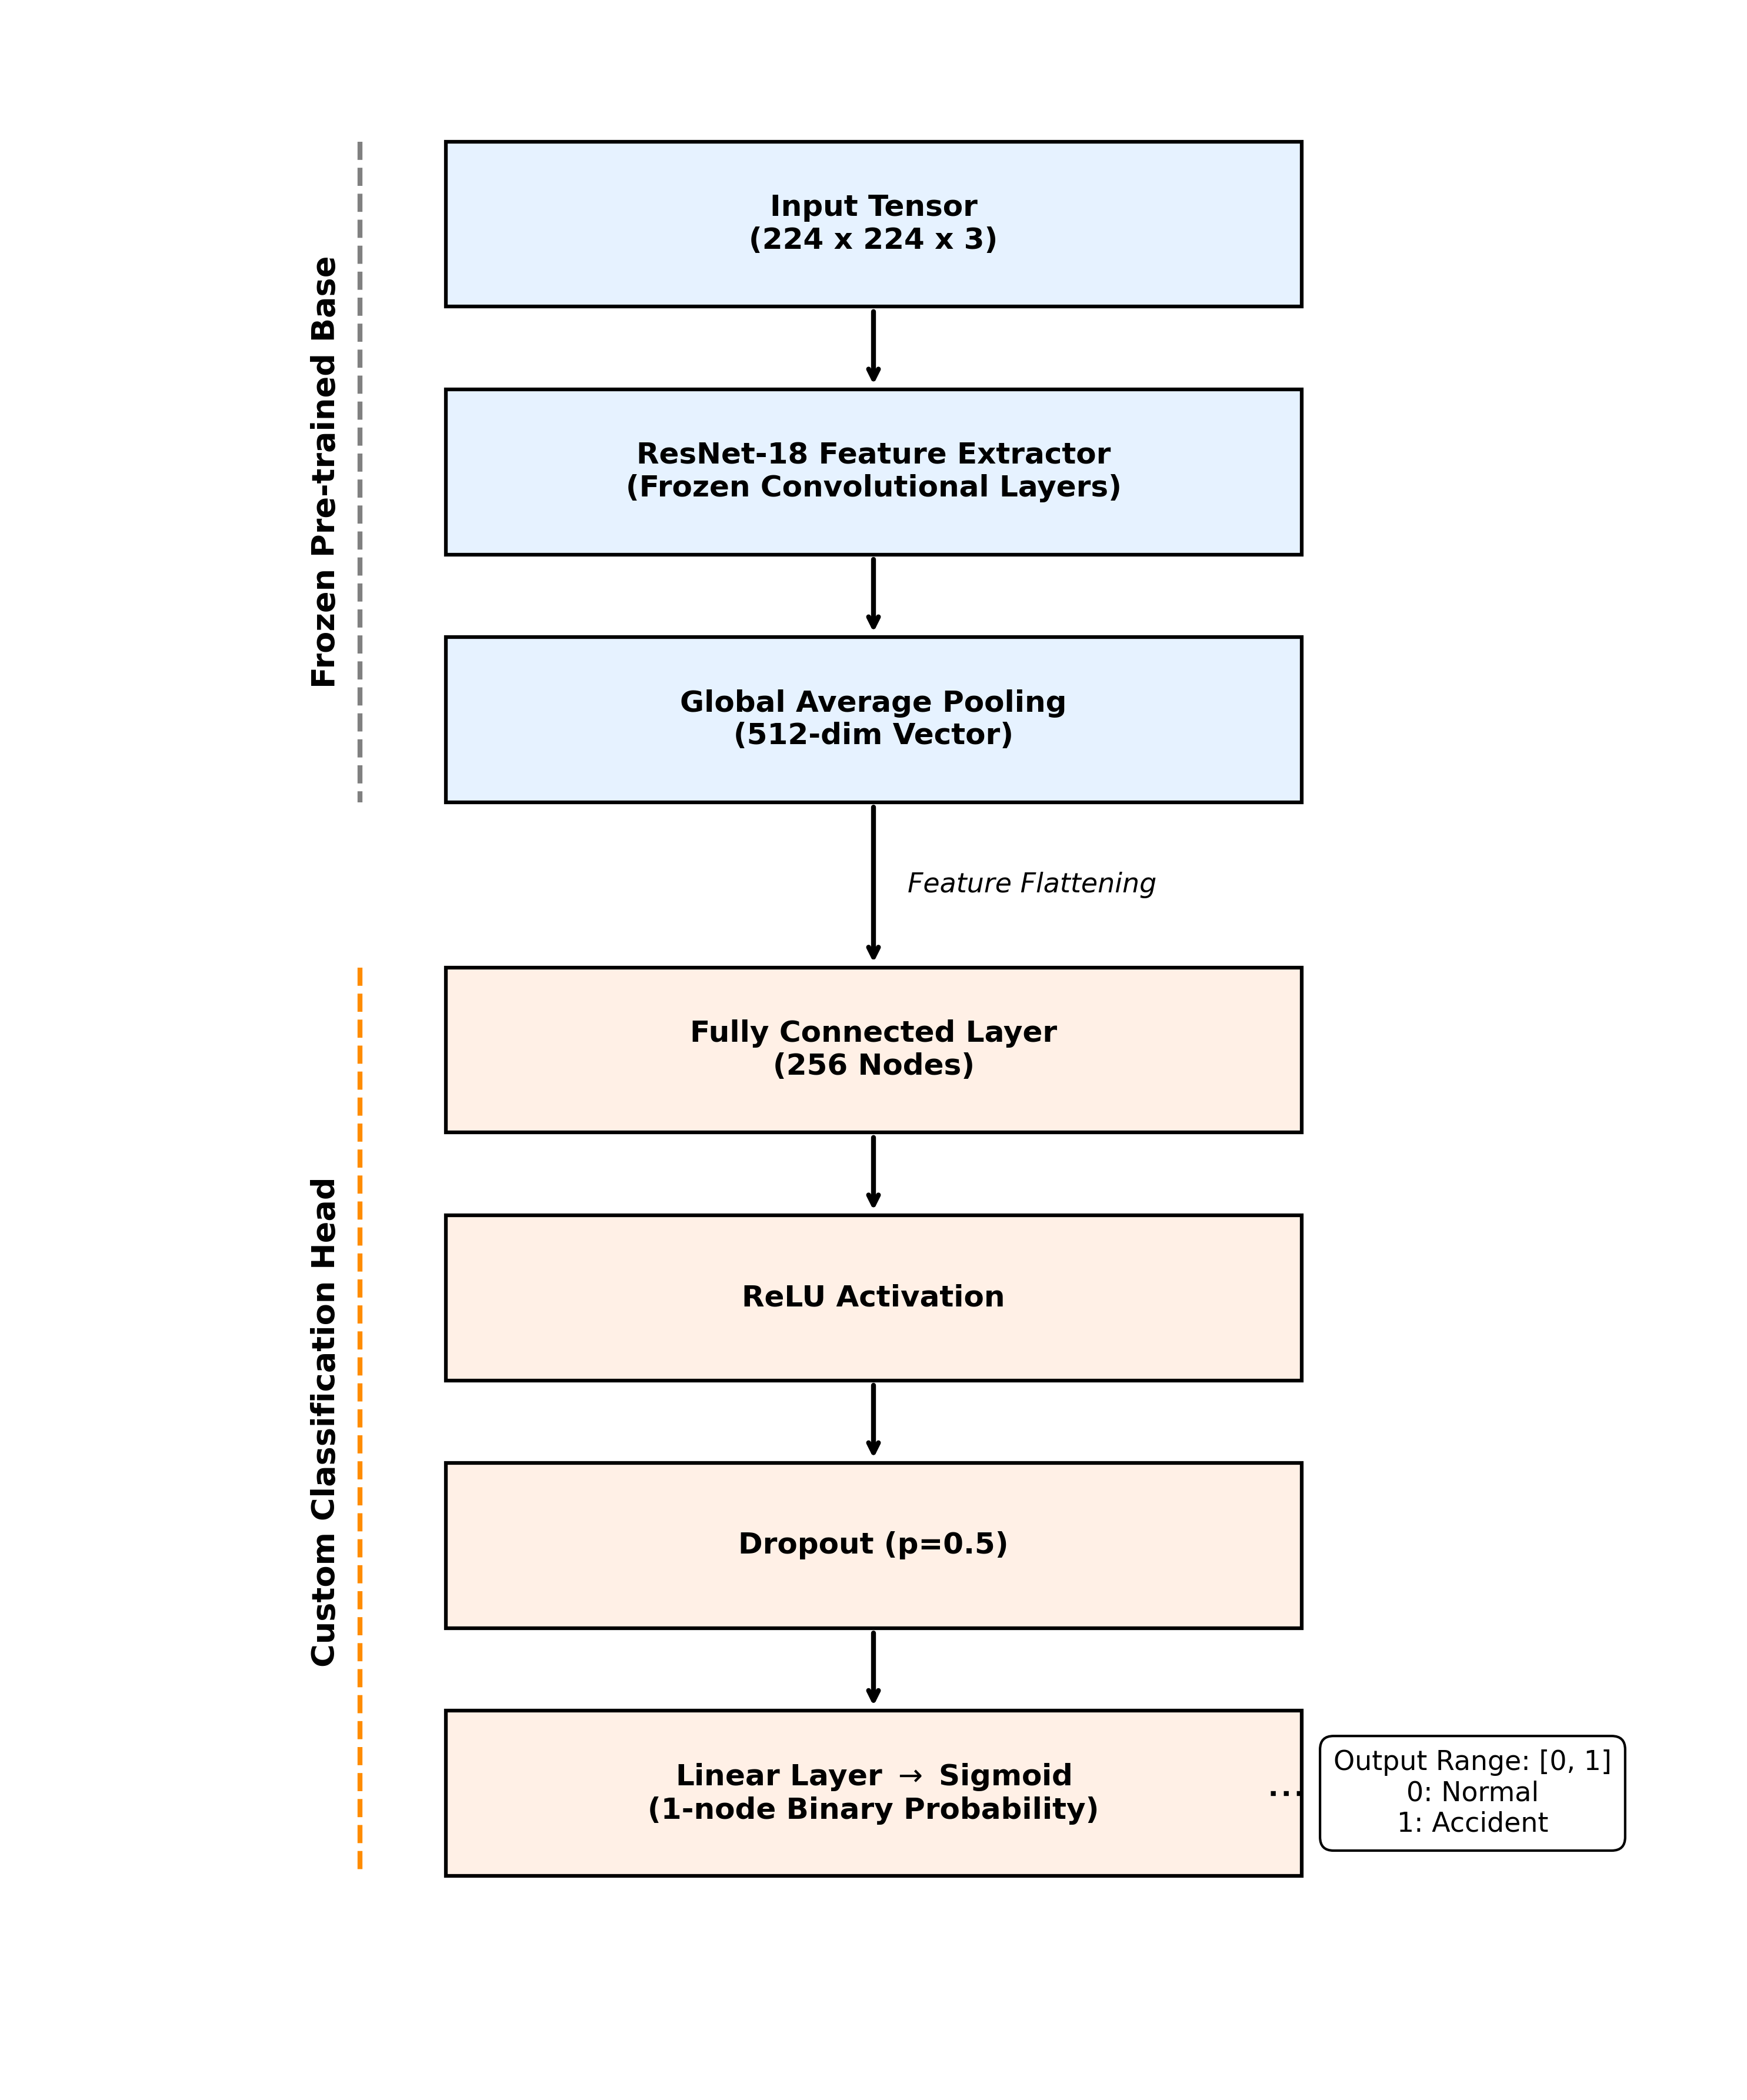
\includegraphics[width=0.8\textwidth]{Figures/resnet_head.png}
    \caption{Diagram of the modified ResNet-18 head, illustrating the frozen convolutional layers passing features into the custom sequential block (256-node Linear $\rightarrow$ ReLU $\rightarrow$ Dropout (0.5) $\rightarrow$ Sigmoid) to generate a binary output.}
    \label{fig:resnet_head}
\end{figure}

To optimise these custom weights, the Binary Cross-Entropy (BCE) loss function was utilised. BCE assesses the probabilistic divergence between the network's continuous Sigmoid output and the discrete ground-truth labels (0 for normal traffic, 1 for an accident). By logarithmically penalising predictions that deviate from the true label, BCE effectively compels the network to refine its boundary delineating normal kinetic flow from chaotic impact signatures.

Training was conducted using the Adam optimiser, set with a learning rate of $0.001$ and a weight decay of $1 \times 10^{-4}$ for structural regularisation. The dataset was processed in batches of 32 images, each resized to $224 \times 224$ pixels and normalised mathematically using the standard ImageNet mean and standard deviation parameters. The network was iteratively trained over twenty epochs, with validation metrics carefully monitored to automatically identify and preserve the highest-performing feature weights for final deployment.

\section{Deep Learning Anomaly Classification}
The HSV-encoded optical flow heatmaps serve as direct input tensors for the deep learning anomaly classifier. To adapt the ResNet-18 architecture for the specific binary classification task of distinguishing between normal traffic flow and serious collisions, the final fully connected layer was modified. It was replaced with a custom sequential block terminating in a Sigmoid activation function, ensuring the network outputs a precise probability score between 0.0 and 1.0.

During the training on the balanced CADP and TAD datasets, the PyTorch optimiser was set up to use a Binary Cross-Entropy (BCE) loss function. This formulation effectively directs the network's optimisation to delineate the precise boundary between standard kinematic activity (such as heavy braking) and the chaotic visual signatures characteristic of a physical impact.

For live deployment, the compiled model weights (\texttt{best\_resnet\_model.pth}) are loaded onto the GPU within a dedicated, asynchronous Python \texttt{ai\_worker} thread. This background worker continuously consumes the pre-processed optical flow frames from the thread-safe \texttt{inference\_queue} and returns a real-time accident probability to the primary physics engine. To stop brief graphical glitches from causing false alarms, the \texttt{main.py} script keeps strict control over the process. The system only kicks in to send an urgent accident alert if the ResNet-18's predicted probability goes over the set threshold (\texttt{CONF\_THRESH = 0.80}) and the number of active pixels exceeds \texttt{PIXEL\_THRESH}, and this happens across 10 consecutive frames.

\section{Inference Pipeline and User Interface}
To transition the trained ResNet-18 model from an experimental framework into a practical operational tool, a live inference pipeline was developed using OpenCV and PyTorch. The inference architecture was explicitly designed to emulate real-world municipal deployment scenarios, wherein continuous video streams must be evaluated sequentially with minimal latency.

The inference loop operates in chronological order. Upon receiving a video feed, the system extracts and buffers the initial frame, converting it into a spatial greyscale matrix. As subsequent frames are streamed into the system, the pipeline continuously computes the dense optical flow between the current frame and the buffered preceding frame. The same transformations employed during training are applied in real-time. This ensures that the continuous video feed is accurately transformed into the precise two-channel, HSV-mapped kinetic pseudo-tensor that the ResNet-18 architecture was trained to interpret.

Once generated, each kinetic tensor is dynamically resized to a resolution of $224 \times 224$ pixels, mathematically normalised using the specified standard deviation parameters, and subsequently processed through the frozen convolutional layers as well as the custom classification head. The network immediately produces a Sigmoid probability score ranging from 0.0 to 1.0.

To bridge the gap between algorithmic processing and human oversight, a streamlined User Interface (UI) was incorporated directly into the video output. A stringent probabilistic safety threshold was defined (for example, 0.50). Should the network’s prediction exceed this threshold, the system promptly signals the presence of anomalous kinetic energy. Visually, the UI superimposes a conspicuous red warning banner, alongside the precise confidence metric directly onto the raw RGB video feed. This approach ensures that, while the neural network analyses the underlying physics of the scene, human emergency operators are provided with an immediate and highly interpretable visual alert to enable swift response coordination.

\begin{figure}[H]
    \centering
    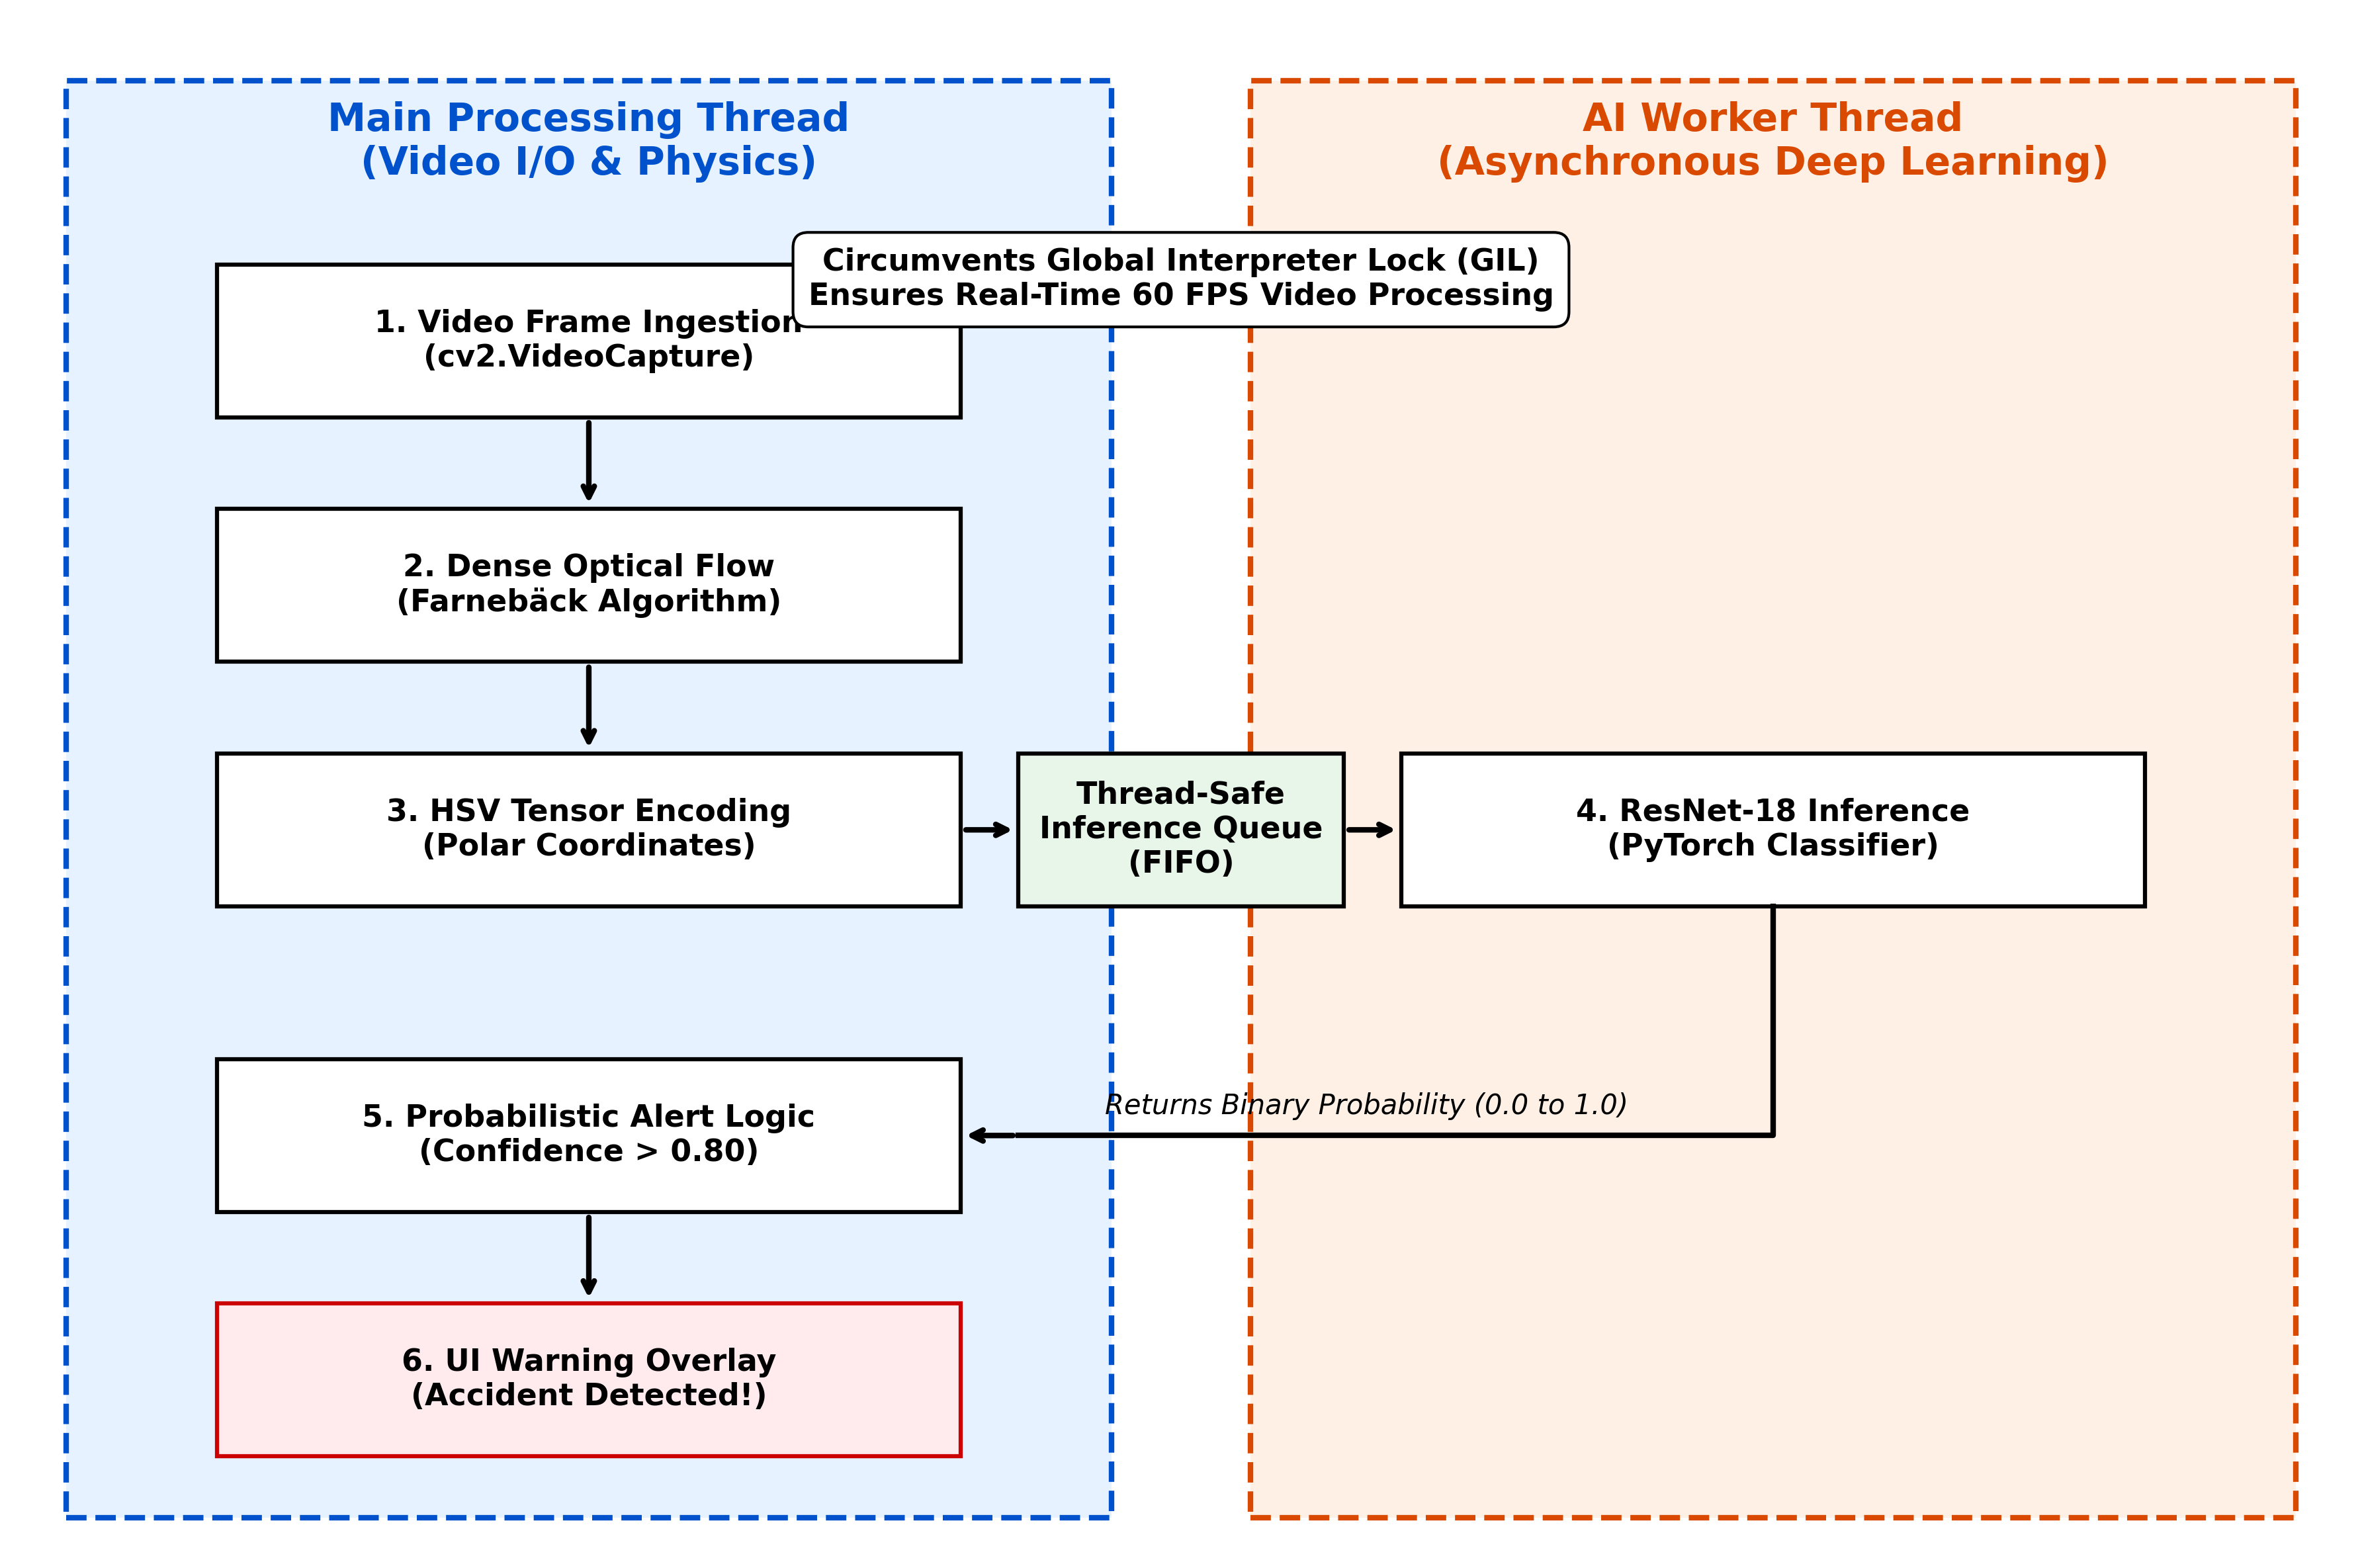
\includegraphics[width=0.9\textwidth]{Figures/system_architecture.png}
    \caption{High-level system architecture detailing the multi-threaded deployment. The main thread manages frame ingestion and Farnebäck optical flow computations, securely transmitting tensors via a thread-safe \texttt{inference\_queue} to the asynchronous \texttt{ai\_worker} thread running the ResNet-18 inference, successfully circumventing the Global Interpreter Lock (GIL).}
    \label{fig:system_architecture}
\end{figure}
\begin{figure}[H]
    \centering
    \begin{minipage}{0.48\textwidth}
        \centering
        
\includegraphics[width=\linewidth]{Figures/dashboard_normal.png}
        \\ \vspace{0.2cm} (a) Normal Traffic Flow
    \end{minipage}\hfill
    \begin{minipage}{0.48\textwidth}
        \centering
        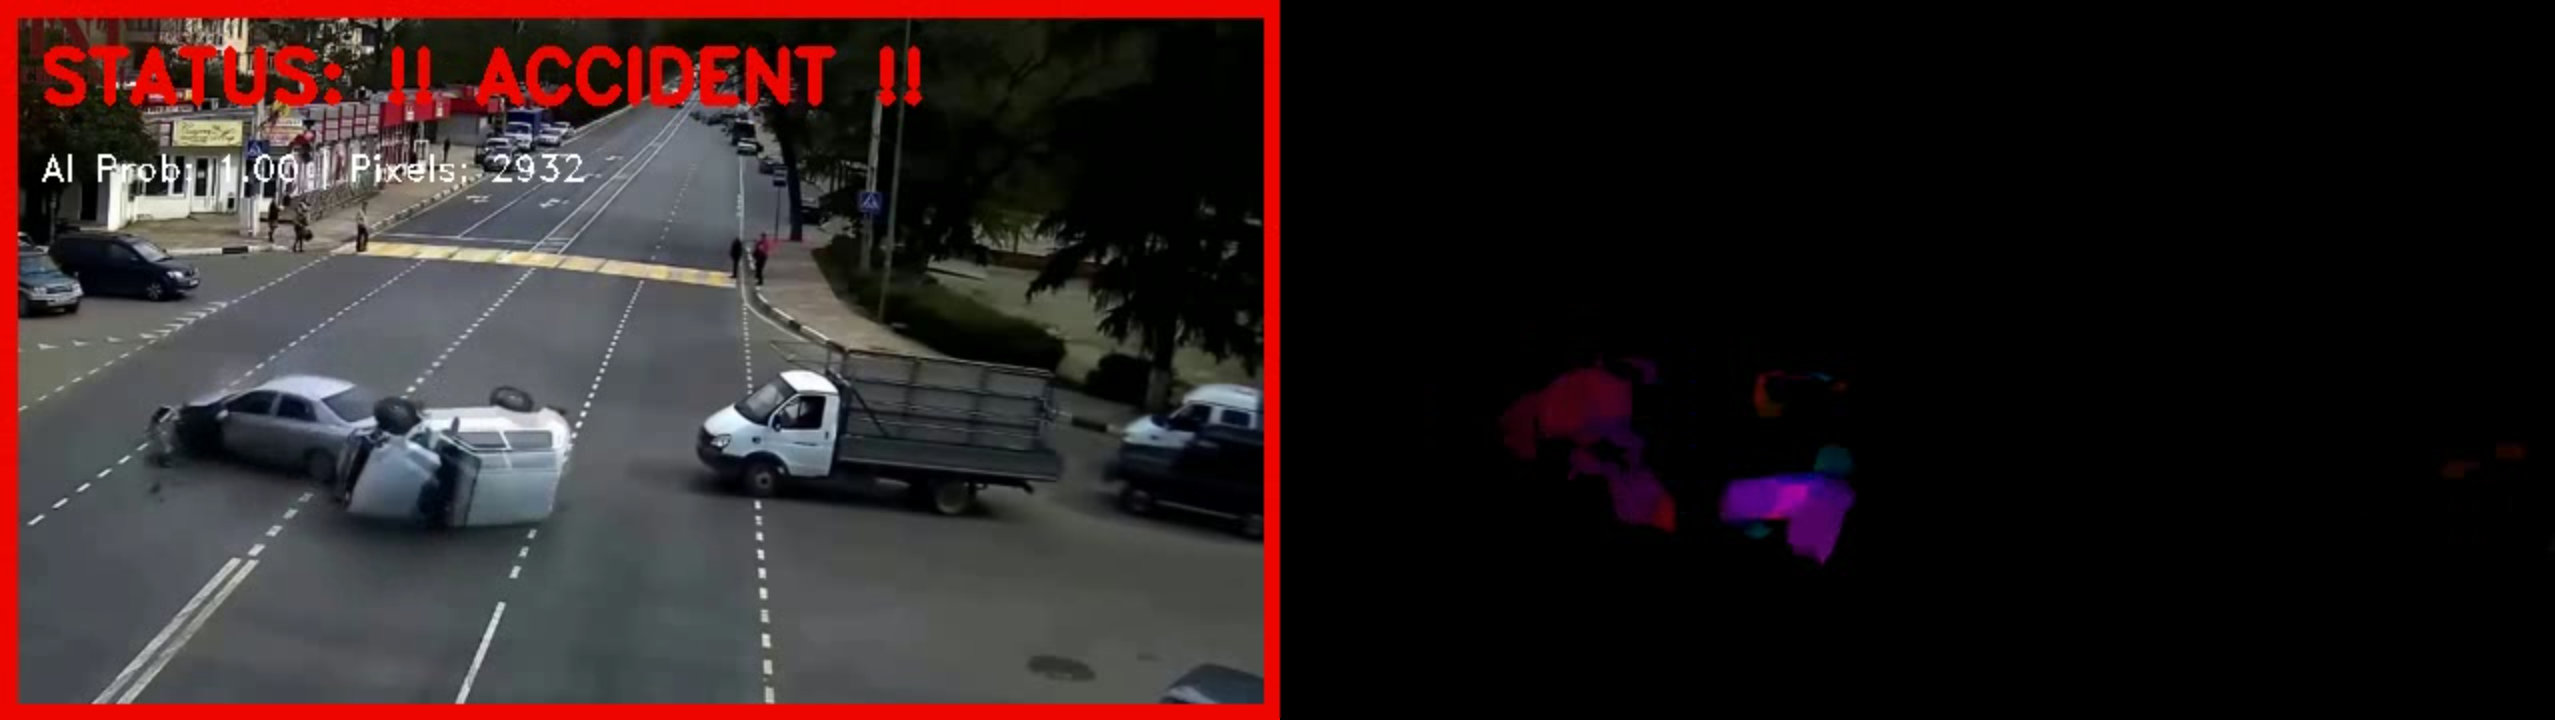
\includegraphics[width=\linewidth]{Figures/dashboard_accident.png}
        \\ \vspace{0.2cm} (b) Accident Detected
    \end{minipage}
    \caption{The real-time Inference User Interface (UI). Panel (a) demonstrates standard operational monitoring with a baseline probability score. Panel (b) illustrates the dynamic red warning overlay triggered when the ResNet-18 confidence metric exceeds the strict safety threshold during a collision.}
    \label{fig:ui_dashboard}
\end{figure}

\section{Evaluation Metrics}
To thoroughly evaluate the performance of the purely spatiotemporal pipeline, a comprehensive quantitative assessment framework was developed. As the system entirely circumvents object detection and speed estimation, conventional metrics such as Mean Average Precision (mAP) or Mean Absolute Error (MAE) are fundamentally unsuitable. Consequently, the evaluation concentrates solely on the classification accuracy of the neural network and the real-time operational efficiency of the system.

The performance of the core anomaly classification is evaluated using precision, recall, and the F1-score. The F1-score was specifically emphasised as the principal Key Performance Indicator (KPI), as it offers a harmonic mean of precision and recall, thereby ensuring the model is rigorously assessed on its capacity to detect rare accidents whilst minimising false positives. Additionally, a Receiver Operating Characteristic (ROC) curve and the corresponding Area Under the Curve (AUC) metric were computed to appraise the robustness of the ResNet-18 classifier across a range of probabilistic thresholds.

To assess the predictive capability of the anomaly module for early-warning deployment, the Time-to-Accident (TTA) metric is employed. This metric quantifies the exact temporal interval (measured in seconds) between the designated alert threshold trigger (\texttt{CONF\_THRESH = 0.80}) and the occurrence of the physical collision. Additionally, the efficiency of the hardware is verified through monitoring the maximum Frames Per Second (FPS) throughput and the total End-to-End Latency, ensuring that the intensive optical flow computations remain within sub-second operational limits.

\begin{table}[H]
    \centering
    \begin{tabular}{p{3cm} p{5cm} p{6cm}}
        \toprule
        \textbf{Metric Category} & \textbf{Assessment Criteria} & \textbf{Key Performance Indicator (KPI)} \\
        \midrule
        Anomaly Classification & Incident Recognition Reliability & F1-Score, Total Accuracy (\%), Precision, Recall \\
        System Robustness & Threshold Independence & ROC Curve, Area under the curve (AUC) \\
        Predictive Capability & Early Warning Responsiveness & Time-to-Accident (TTA) \\
        System Optimisation & Real-time Throughput & Frames Per Second (FPS), End-to-End Latency (ms) \\
        \bottomrule
    \end{tabular}
    \caption{Evaluation Metrics for the Spatiotemporal Architecture}
    \label{tab:evaluation_metrics}
\end{table}
\end{spacing}
\newpage
